blablabla
\begin{thm}
    \textcolor{red}{round decompose locally semicomplete digraph}
\end{thm}
Every locally semicomplete digraph can be classified into some other groups of digraphs namely semicomplete digraphs and round decomposable digraphs and the last one which is neither of the two is call evil. Round decomposable digraph $D=R[D_1,\dots,D_r]$ is where $R$ is a round digraph of the strong componentents $D_i$ and $|R|=r$.
\begin{thm}~\cite{bangJGT85}
    Let $D$ be a locally semicomplete digraph. Then exactly one of the following possibilities holds. Furthermore, there is a polynomial algorithm that decides which of the properties hold and gives a certificate for this.
    \begin{itemize}
        \item[(a)] $D$ is round decomposable with a unique round decomposition $R[D_1,\dots ,D_r]$, where $R$ is a round local tournament on $r\geq 2$vertices and $D_i$ is strong semicomplete digraph for $i=1,2,\dots,r$.
        \item[(b)] $D$ is evil 
        \item[(c)] $D$ is a semicomplete digraph thet is not round decomposable. 
    \end{itemize}
\end{thm}
If the locally semicomplete digraph is nonstrong it turns out that it is decomposable this is called a semicomplete decomposition.
\begin{thm}~\cite{bangJGT85,banggutin,bangJCT102}
    Let $D$ be a nonstrong locally semicomplete digraph and let $D_1,D_2,\dots,D_p$ be the acyclic order of the strong components of $D$. Then $D$ can be decomposed into $r\geq 2$ disjoint subdigraphs $D_1',D_2',\dots, D_r'$ as follows:
    \begin{align*}
        D_1'=D_p, \lambda_1=p,\\
        \lambda_{i+1}=min\lbrace j|N^+(D_j)\cap V(D'_i)\neq \emptyset\rbrace,
    \end{align*}
    and
    \begin{equation*}
        D'_{i+1}=D\left<V(D_{lambda_{i+1}})\cup V(D_{lambda_{i+1}+1})\cup \cdots \cup V(D_{lambda_{i}-1})\right>
    \end{equation*}
    The subdigraphs $D'_1,D'_2,\dots,D'_r$ satisfy the properties below:
    \begin{itemize}
        \item[(a)] $D'_i$ consists of some strong components that are consecutive in the acyclic ordering of the strong components of $D$ and is semicomplete for $1=1,2,\dots,r$;
        \item[(b)] $D'_{i+1}$ dominates the initial component of $D'_i$ and there exists no arc from $D'_i$ to $D'_{i+1}$ for $i=1,2,\dots,r-1$;
        \item[(c)] if $r\geq 3$ then there exists no arc between $D'_i$ and $D'_j$ for $i,j$ satisfying $|j-i|\geq 2$  
    \end{itemize}
    \label{thm:semicompletedecom}
\end{thm}
For simplification of \autoref{thm:semicompletedecom} the properties is drawn out in \autoref{fig:properties}
\begin{figure}
    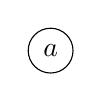
\begin{tikzpicture}[main/.style ={draw,circle}]
        \node[main](a){$a$};
    \end{tikzpicture}
    \caption{(a)(b) and (c)}
    \label{fig:properties}
\end{figure}
Now we focus more on the structure of the evil locally semicomplete digraph which we have not covered jet, there is a fine understanding of the structure of round decomposable and the semicomplete digraphs, even the semicomplete decomposition which is a part of the evil structure too.
First we have to recall what a minimal seperator from \autoref{sec:digraph}, then use this to construct what we call a \textbf{good} seperator.
\begin{lemma}~\cite{bangJGT85}
    Let $S$ ba a minimal seperator of the locally semicomplete digraph $D$. Then either $D\left< S\right>$ is semicomplete or $D\left< V-S\right>$ is semicomplete.
    \label{lem:whichsemicomplete}
\end{lemma}
Then a \textbf{good} seperator of a locally semicomplete digraph is minimal and $D\left<V-S\right>$ is not semicomplete.
When finding a good seperator in a evil locally semicomplete digraph, then the part that is left $D-S$ a semicomplete decomposition can be found it turns out that there is a lot to say about this decomposition.
\begin{thm}~\cite{bangJGT85,bangJCT102}
    Let $D$ be an evil locally semicomplete digraph then $D$ is strong and satisfies the following properties.
    \begin{itemize}
        \item[(a)]There is a good seperator S such that the semicomplete decomposition of $D-S$ has exactly three components $D'_1,D'_2,D'_3$ (and $D\left<S\right>$ is semicomplete by \autoref{lem:whichsemicomplete});
        \item[(b)] Furthermore, for each such $S$, there are integers $\alpha, \beta,\mu,\nu$ with $\lambda_2\leq \alpha \leq \beta \leq p-1$ and $p+1\leq \mu \leq \nu \leq p+q$ such that 
        \begin{align}
            &N^-(D_\alpha)\cap V(D_\mu)\neq \emptyset \text{and} N^+(D_\alpha)\cap V(D_\nu)\neq \emptyset,\\
            \text{or} &N^-(D_\mu)\cap V(D_\alpha)\neq \emptyset \text{and} N^+(D_\mu)\cap V(D_\beta)\neq \emptyset,
        \end{align} 
        where $D_1,D_2,\dots, D_p$ and $D_{p+1},\dots,D_{p+q}$ are the strong decomposition of $D-S$ and $D\left< S\right>$, respectively, and $D_{\lambda_2}$is the initial component of $D'_2$ 
    \end{itemize}
    \label{thm:evildecom}
\end{thm}
Even though this is a structure we can work with, we can actually go deeper into the structure of this evil locally semicomplete digraph. Namly trying to group the components inside the semicomplete decomposition $D'_1,D'_2,D'_3$ and the good seperator $S$. This structer is menation in \cite{bangJGT85} but also in \cite{tildeDMCS}. First we can establish this lemma which is a big part of the structure of evil locally semicomplete digraphs.
\begin{lemma}~\cite{tildeDMCS}
    Let $D$ be an evil locally semicomplete digraph and let $S$ be a good seperator od $D$. Then the following holds:
    \begin{itemize}
        \item[(i)] $D_p\Rightarrow S\Rightarrow D_1$.
        \item[(ii)] If $sv$ is an arc from $S$ to $D'_2$ with $s\in V(D_i)$ and $v\in V(D_j)$, then 
        \begin{equation*}
            D_i\cup D_{i+1}\cup \dots D_{p+q}\Rightarrow D_1\cup\dots \cup D_{\lambda_2-1}\Rightarrow D_{\lambda_2}\cup \dots \cup D_j
        \end{equation*}.
        \item[(iii)] $D_{p+q}\Rightarrow D'_3$ and $D_f\Rightarrow D_{f+1}$ for $f\in [p+q]$, where $p+q+1=1$.
        \item[(iv)] If there is any arc from $D_i$ to $D_j$ with $i\in [\lambda_2-1]$ and $j\in [\lambda_2,p-1]$, then $D_a\Rightarrow D_b$ for all $a\in [i,\lambda_2-1]$ and $b\in[\lambda_2,j]$.
        \item[(v)] If there is any arc from $D_k to D_l$ with $k\in [p+1,p+q]$ and $l\in [\lambda_2-1]$, then $D_a\Rightarrow D_b$ for all $a\in [k,p+q]$ and $b\in [l]$.   
    \end{itemize}
\end{lemma}
